%%%%%%%%%%%%%%%%%%%%%%%%%%%%%%%%%%%%%%%%%
% Programming/Coding Assignment
% LaTeX Template
%
% This template has been downloaded from:
% http://www.latextemplates.com
%
% Original author:
% Ted Pavlic (http://www.tedpavlic.com)
%
% Note:
% The \lipsum[#] commands throughout this template generate dummy text
% to fill the template out. These commands should all be removed when 
% writing assignment content.
%
% This template uses a Perl script as an example snippet of code, most other
% languages are also usable. Configure them in the "CODE INCLUSION 
% CONFIGURATION" section.
%
%%%%%%%%%%%%%%%%%%%%%%%%%%%%%%%%%%%%%%%%%

%----------------------------------------------------------------------------------------
%	PACKAGES AND OTHER DOCUMENT CONFIGURATIONS
%----------------------------------------------------------------------------------------

\documentclass{article}

\usepackage{fancyhdr} % Required for custom headers
\usepackage{lastpage} % Required to determine the last page for the footer
\usepackage{extramarks} % Required for headers and footers
\usepackage[usenames,dvipsnames]{color} % Required for custom colors
\usepackage{graphicx} % Required to insert images
\usepackage{listings} % Required for insertion of code
\usepackage{courier} % Required for the courier font
\usepackage{lipsum} % Used for inserting dummy 'Lorem ipsum' text into the template
\usepackage{multicol} 

\usepackage{tikz}
\usetikzlibrary{arrows,calc} 

\usepackage{fancyvrb}

% redefine \VerbatimInput
\RecustomVerbatimCommand{\VerbatimInput}{VerbatimInput}%
{
    fontsize=\footnotesize,
    %
    frame=lines,  % top and bottom rule only
    framesep=2em, % separation between frame and text
    rulecolor=\color{Gray},
    %
    label=\fbox{\color{Black}JavaImplementationOutput.txt},
    labelposition=topline,
    %
    commandchars=\|\(\), % escape character and argument delimiters for
    % commands within the verbatim
    commentchar=*        % comment character
}

\usepackage{quoting}
\quotingsetup{vskip=0pt}

\usepackage[plain]{algorithm}
\usepackage{algpseudocode}
\usepackage{subcaption}

\usepackage{mathtools}
\usepackage{amsmath, amsthm, amssymb}
\usepackage[ansinew]{inputenc}

\makeatletter
\renewcommand{\boxed}[1]{\text{\fboxsep=.2em\fbox{\m@th$\displaystyle#1$}}}
\makeatother

% Margins
\topmargin=-0.45in
\evensidemargin=0in
\oddsidemargin=0in
\textwidth=6.5in
\textheight=9.0in
\headsep=0.25in

\linespread{1.1} % Line spacing

% Set up the header and footer
\pagestyle{fancy}
\lhead{\hmwkAuthorName} % Top left header
\chead{\hmwkClass: \hmwkTitle} % Top center head
\rhead{}
\cfoot{} % Bottom center footer
\rfoot{Page\ \thepage\ of\ \protect\pageref{LastPage}} % Bottom right footer
\renewcommand\headrulewidth{0.4pt} % Size of the header rule
\renewcommand\footrulewidth{0.4pt} % Size of the footer rule

\setlength\parindent{0pt} % Removes all indentation from paragraphs

%----------------------------------------------------------------------------------------
%	CODE INCLUSION CONFIGURATION
%----------------------------------------------------------------------------------------

\definecolor{MyDarkGreen}{rgb}{0.0,0.4,0.0} % This is the color used for comments
\lstloadlanguages{Perl} % Load Perl syntax for listings, for a list of other languages supported see: ftp://ftp.tex.ac.uk/tex-archive/macros/latex/contrib/listings/listings.pdf
\lstset{language=Perl, % Use Perl in this example
        frame=single, % Single frame around code
        basicstyle=\small\ttfamily, % Use small true type font
        keywordstyle=[1]\color{Blue}\bf, % Perl functions bold and blue
        keywordstyle=[2]\color{Purple}, % Perl function arguments purple
        keywordstyle=[3]\color{Blue}\underbar, % Custom functions underlined and blue
        identifierstyle=, % Nothing special about identifiers                                         
        commentstyle=\usefont{T1}{pcr}{m}{sl}\color{MyDarkGreen}\small, % Comments small dark green courier font
        stringstyle=\color{Purple}, % Strings are purple
        showstringspaces=false, % Don't put marks in string spaces
        tabsize=5, % 5 spaces per tab
        %
        % Put standard Perl functions not included in the default language here
        morekeywords={rand},
        %
        % Put Perl function parameters here
        morekeywords=[2]{on, off, interp},
        %
        % Put user defined functions here
        morekeywords=[3]{test},
       	%
        morecomment=[l][\color{Blue}]{...}, % Line continuation (...) like blue comment
        numbers=left, % Line numbers on left
        firstnumber=1, % Line numbers start with line 1
        numberstyle=\tiny\color{Blue}, % Line numbers are blue and small
        stepnumber=5 % Line numbers go in steps of 5
}

% Creates a new command to include a perl script, the first parameter is the filename of the script (without .pl), the second parameter is the caption
\newcommand{\perlscript}[2]{
\begin{itemize}
\item[]\lstinputlisting[caption=#2,label=#1]{#1.pl}
\end{itemize}
}

%----------------------------------------------------------------------------------------
%	DOCUMENT STRUCTURE COMMANDS
%	Skip this unless you know what you're doing
%----------------------------------------------------------------------------------------

% Header and footer for when a page split occurs within a problem environment
\newcommand{\enterProblemHeader}[1]{
\nobreak\extramarks{#1}{#1 continued on next page\ldots}\nobreak
\nobreak\extramarks{#1 (continued)}{#1 continued on next page\ldots}\nobreak
}

% Header and footer for when a page split occurs between problem environments
\newcommand{\exitProblemHeader}[1]{
\nobreak\extramarks{#1 (continued)}{#1 continued on next page\ldots}\nobreak
\nobreak\extramarks{#1}{}\nobreak
}

\setcounter{secnumdepth}{0} % Removes default section numbers
\newcounter{homeworkProblemCounter} % Creates a counter to keep track of the number of problems

\newcommand{\homeworkProblemName}{}
\newenvironment{homeworkProblem}[1][Question \arabic{homeworkProblemCounter}]{ % Makes a new environment called homeworkProblem which takes 1 argument (custom name) but the default is "Problem #"
\stepcounter{homeworkProblemCounter} % Increase counter for number of problems
\renewcommand{\homeworkProblemName}{#1} % Assign \homeworkProblemName the name of the problem
\section{\homeworkProblemName} % Make a section in the document with the custom problem count
\enterProblemHeader{\homeworkProblemName} % Header and footer within the environment
}{
\exitProblemHeader{\homeworkProblemName} % Header and footer after the environment
}

\newcommand{\problemAnswer}[1]{ % Defines the problem answer command with the content as the only argument
\noindent\framebox[\columnwidth][c]{\begin{minipage}{0.98\columnwidth}#1\end{minipage}} % Makes the box around the problem answer and puts the content inside
}

\newcommand{\homeworkSectionName}{}
\newenvironment{homeworkSection}[1]{ % New environment for sections within homework problems, takes 1 argument - the name of the section
\renewcommand{\homeworkSectionName}{#1} % Assign \homeworkSectionName to the name of the section from the environment argument
\subsection{\homeworkSectionName} % Make a subsection with the custom name of the subsection
\enterProblemHeader{\homeworkProblemName\ [\homeworkSectionName]} % Header and footer within the environment
}{
\enterProblemHeader{\homeworkProblemName} % Header and footer after the environment
}

%----------------------------------------------------------------------------------------
%	NAME AND CLASS SECTION
%----------------------------------------------------------------------------------------

\newcommand{\hmwkTitle}{Assignment\ \#1} % Assignment title
\newcommand{\hmwkDueDate}{Monday, 16\textsuperscript{th} of May, 2016} % Due date
\newcommand{\hmwkClass}{Design and Analysis of Algorithms} % Course/class
\newcommand{\hmwkClassTime}{4:00pm} % Class/lecture time
\newcommand{\hmwkClassInstructor}{Jones} % Teacher/lecturer
\newcommand{\hmwkAuthorName}{Tim Cochrane} % Your name
\newcommand{\studentNum}{17766247}

%----------------------------------------------------------------------------------------
%	TITLE PAGE
%----------------------------------------------------------------------------------------

\title{
\vspace{2in}
\textmd{\textbf{\hmwkClass}}\\
\textmd{\hmwkTitle}\\
\normalsize\vspace{0.1in}\small{\hmwkDueDate}\\
\vspace{3in}
}

\author{\textbf{\hmwkAuthorName} \\ \studentNum}
\date{} % Insert date here if you want it to appear below your name

%----------------------------------------------------------------------------------------

\begin{document} 
\maketitle\thispagestyle{empty}

%----------------------------------------------------------------------------------------
%	TABLE OF CONTENTS
%----------------------------------------------------------------------------------------

%\setcounter{tocdepth}{1} % Uncomment this line if you don't want subsections listed in the ToC

%  \newpage
%  \tableofcontents
%  \newpage

\clearpage
\setcounter{page}{1}

%----------------------------------------------------------------------------------------
%	PROBLEM 1
%----------------------------------------------------------------------------------------

% To have just one problem per page, simply put a \clearpage after each problem

\begin{homeworkProblem}

    a) Use the Master method solve the folloing recurrence function:
    \begin{center}
        $T(n) = 3T(\sqrt[2]{n}) + \log_2{n}$
    \end{center}
    \textbf{Solution}
    \begin{quoting}
        \abovedisplayskip=0pt
        \begin{align}
            \shortintertext{Inital recurance:}
            T(n) & = 3T(\sqrt[2]{n}) + \log_2{n} \notag \\
            \shortintertext{Substitute for $k = \log_2{n}$:}
            T(2^k) & = 3T(2^{\frac{k}{2}}) + k \notag \\
            \shortintertext{Now in the master thereom form:}
            T(n) & = aT(n/b) + f(n) \notag \\
            \shortintertext{Where:}
            a = 3, b & = 2, f(n) = k \notag
            \shortintertext{Checking which master thereom case to use:}
            k^{\log_b{a}} & = k^{\log_2{3}} \approx k^{1.6} \notag \\
            k^{1} & < k^{1.6} \notag
        \end{align}
        \begin{center}
            $\therefore$ case 1 of master thereom \\
            The solution to the recurance is $O(n^{\log_2{3}})$.
        \end{center}
    \end{quoting}
    \vskip0.5cm
   %\begin{align}
   %    \sqrt{k} = \sqrt{\log_2{n}} = 2^{\frac{\log_2{n}}{2}} = 2^\frac{k}{2}
   %\end{align}

    b) Consider the recurrence function $T(n) = 2T(n-1)+1$ state the upper 
    bound time complexity of the function and use induction to 
    prove that the time complexity is correct. \\

    \textbf{Solution}

    \begin{quoting}
        Assuming that $T(1) = 1$ lets calculate the first few values of the
        the recurrance to get an idea of the function.
        \begin{align}
            T(1) & = 1 \notag \\
            T(2) & = 2(1) + 1 = 3 \notag \\
            T(3) & = 2(3) + 1 = 7 \notag \\
            T(4) & = 2(7) + 1 = 15 \notag
        \end{align}

        The initial values of the recurrance appears to be $2^{n} - 1$. Lets
        try and prove this by induction. \\

        \textbf{Inductive Hypothesis}
        \begin{center}
            $T(n) \in O(2^{n} - 1)$
        \end{center}
        \textbf{Base Case}
        \begin{align}
            T(2) & = 2T(2 - 1) + 1 & 2^{2} - 1 & = 4 - 1 \notag \\
                 & = 2T(1) + 1 & & = 3 \notag \\
                 & = 2 + 1 = 3 & & = 3 \notag
        \end{align}
        \begin{center}
            $\therefore$ \text{base case holds}
        \end{center}

        \textbf{Inductive Step}
        \begin{align}
            T(n + 1) & = 2T(n + 1 - 1) + 1 \notag \\
                     & = 2T(n) + 1 \notag \\
                     & = 2(2^{n} - 1) + 1 \notag \\
                     & = 2^{n+1} - 2 + 1 \notag \\
                     & = 2^{n+1} - 1 \notag 
        \end{align}
        \begin{center}
            Same form as our hypothesis
        \end{center}
        \vskip0.5cm
        We have proven through induction that the recurance has an upper 
        bound time complexity of $O(2^n)$.
    \end{quoting}

\end{homeworkProblem}

%----------------------------------------------------------------------------------------
%	PROBLEM 2
%----------------------------------------------------------------------------------------

\begin{homeworkProblem}
    \begin{figure}[H]
        \begin{center}
            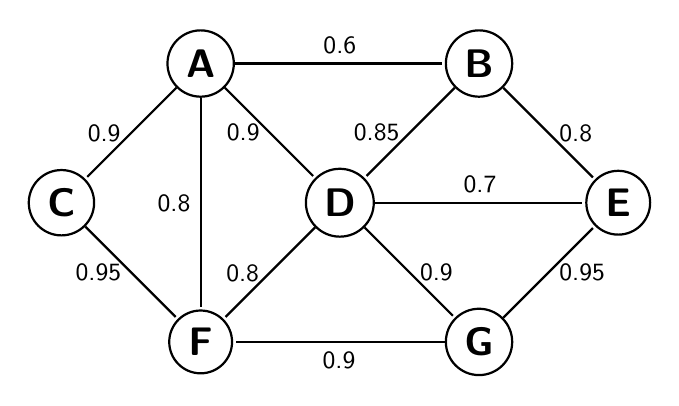
\begin{tikzpicture}[>=stealth',shorten >=1pt,auto,node distance=2.5cm,
                thick,main node/.style={circle,draw,font=\sffamily\Large\bfseries}]

                \node[main node] (A) {A};
                \node[main node] (D) [below right of=A]{D};
                \node[main node] (B) [above right of=D]{B};
                \node[main node] (C) [below left of=A]{C};
                \node[main node] (E) [below right of=B]{E};
                \node[main node] (F) [below left of=D]{F};
                \node[main node] (G) [below right of=D]{G};

                \path[every node/.style={font=\sffamily\small}]
                (A) edge node [left] {0.9} (C)
                    edge node [left] {0.8} (F)
                    edge node [left] {0.9} (D)
                    edge node [above] {0.6} (B)
                (B) edge node [left] {0.85} (D)
                    edge node [right] {0.8} (E)
                (C) edge node [left] {0.95} (F)
                (D) edge node [above] {0.7} (E)
                    edge node [right] {0.9} (G)
                    edge node [left] {0.8} (F)
                (G) edge node [below] {0.9} (F)
                    edge node [right] {0.95} (E);
            \end{tikzpicture}
        \end{center}
        \caption{Undirected weighted graph}
        \belowcaptionskip0cm
        \label{graph1}
    \end{figure}

    a) Design a \textit{greedy} algorithm that generates the most reliable path from
    a source node $s$ to every destination node $t$ in the network. Show your algorithm
    in a concise and clear pseudo-code. Further, you must explain in detail each line
    of your pseudo-code and show how to implement your algorithm so that it has the
    best possible time complexity. \\

    \textbf{Solution}
    \begin{algorithm}[H]
        \begin{algorithmic}[1]
            \Function{Dijkstra}{$G, w, s$}
            \State{} \Call{Initialize-Single-Source}{$G, s$}
            \State{} $S = \emptyset$
            \State{} $Q = G.V$
                \While{$Q \neq \emptyset$}
                    \State{} $u = \Call{Extract-Max}{$Q$} $
                    \State{} $S = S \cup \{u\}$
                    \For{each vertex $v \in G.Adj[u]$}
                        \State{} \Call{Tense}{$u,v,w$}
                    \EndFor
                \EndWhile \EndFunction{}
        \end{algorithmic}
        \caption{Modified Dijkstra's Algorithm}
        \label{alg:path}
    \end{algorithm}
    \begin{algorithm}[H]
        \begin{algorithmic}[1]
            \Function{Initialize-Single-Source}{$G, s$}
                \For{each vertex $v \in G.V$}
                    \State{} $v.d = \infty$
                    \State{} $v.\pi = NIL$
                \EndFor
            \State{} $s.d = 1$
            \EndFunction
        \end{algorithmic}
        \caption{Initialize our vertex's}
    \end{algorithm}
    \begin{algorithm}[H]
        \begin{algorithmic}[1]
            \Function{Tense}{$u, v, w$}
                \If{$v.d < u.d * w(u,v)$}
                    \State{} $v.d = u.d * w(u,v)$
                    \State{} $v.\pi = u$
                \EndIf
            \EndFunction{}
        \end{algorithmic}
        \caption{Modified Relax Algorithm}
    \end{algorithm}

    \vskip0.5cm

    b) Use your algorithm in part a) to generate the most reliable path from
    node A to every other node for the given graph. List the most reliable paths and
    their corresponding path reliabilities. 

    \begin{figure}[H]
        \begin{center}
            \begin{tabular}{*{8}{c |}}
                & $A$ & $B$ & $C$ & $D$ & $E$ & $F$ & $G$ \\
            \hline
        $A$ & $\boxed{1}$ & $0.6$ & $0.9$ & $0.9$ & $\infty$ & $0.8$ & $\infty$ \\
        $C$ & $1$ & $0.6$ & $\boxed{0.9}$ & $0.9$ & $\infty$ & $0.855$ & $\infty$ \\
        $D$ & $1$ & $0.765$ & $0.9$ & $\boxed{0.9}$ & $0.63$ & $0.855$ & $0.81$ \\
        $F$ & $1$ & $0.765$ & $0.9$ & $0.9$ & $0.63$ & $\boxed{0.855}$ & $0.81$ \\
        $G$ & $1$ & $0.765$ & $0.9$ & $0.9$ & $0.7695$ & $0.8$ & $\boxed{0.81}$ \\
        $E$ & $1$ & $0.765$ & $0.9$ & $0.9$ & $\boxed{0.7695}$ & $0.8$ & $0.81$ \\
        $B$ & $1$ & $\boxed{0.765}$ & $0.9$ & $0.9$ & $0.7695$ & $0.8$ & $0.81$ \\
            \end{tabular}
            \caption{Result of Algorithm~\ref{alg:path}}
            \label{path_result}
        \end{center}
    \end{figure}

    \begin{quoting}
        From the algorithm we have found the following paths to each node:
        \begin{align}
            B:&  \{A \to D \to B\} = 0.765 \notag \\
            C:&  \{A \to C\} = 0.9  \notag \\
            D:&  \{A \to D\} = 0.9  \notag \\
            E:&  \{A \to D \to G \to E\} = 0.7695 \notag \\
            F:&  \{A \to C \to F \} = 0.855 \notag \\
            G:&  \{A \to D \to G \} = 0.81 \notag
        \end{align}
    \end{quoting}
\end{homeworkProblem}

%----------------------------------------------------------------------------------------

\begin{homeworkProblem}
    \begin{figure}[H]
        \begin{center}
            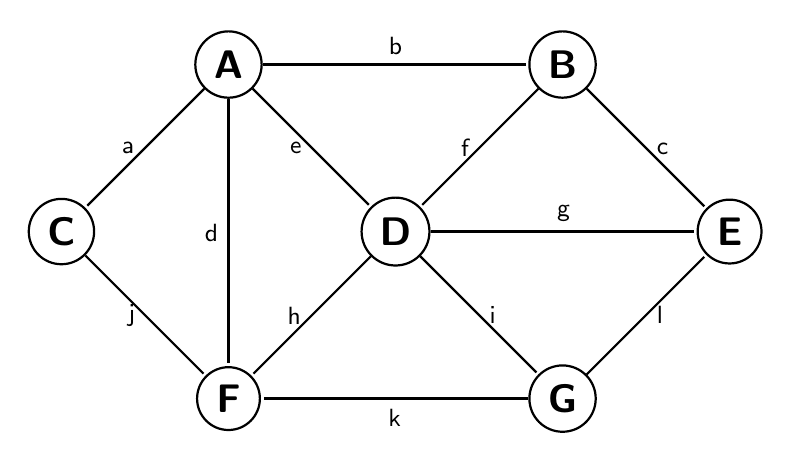
\begin{tikzpicture}[>=stealth',shorten >=1pt,auto,node distance=3cm,
                thick,main node/.style={circle,draw,font=\sffamily\Large\bfseries}]

                \node[main node] (A) {A};
                \node[main node] (D) [below right of=A]{D};
                \node[main node] (B) [above right of=D]{B};
                \node[main node] (C) [below left of=A]{C};
                \node[main node] (E) [below right of=B]{E};
                \node[main node] (F) [below left of=D]{F};
                \node[main node] (G) [below right of=D]{G};

                \path[every node/.style={font=\sffamily\small}]
                (A) edge node [left] {a} (C)
                    edge node [left] {d} (F)
                    edge node [left] {e} (D)
                    edge node [above] {b} (B)
                (B) edge node [left] {f} (D)
                    edge node [right] {c} (E)
                (C) edge node [left] {j} (F)
                (D) edge node [above] {g} (E)
                    edge node [right] {i} (G)
                    edge node [left] {h} (F)
                (G) edge node [below] {k} (F)
                    edge node [right] {l} (E);
            \end{tikzpicture}
        \end{center}
        \caption{Undirected weighted graph}
        \belowcaptionskip0cm
        \label{graph2}
    \end{figure}

    a) Generate all possible cuts in the given graph, and determine its
    maximum cut. \\

    \begin{quoting}
        After generating all of the possible cuts, I found the largest cut
        had a size of 9 and occured with the following subsets.

        \begin{center}
            $s_1 = \{B,C,D,G\}, s_2 = \{A,E,F\}$
        \end{center}

        The order of these subsets is irrelivent as flipping the variables
        will still produce the same cut. \\


        \begin{figure}[H]
            \begin{center}
                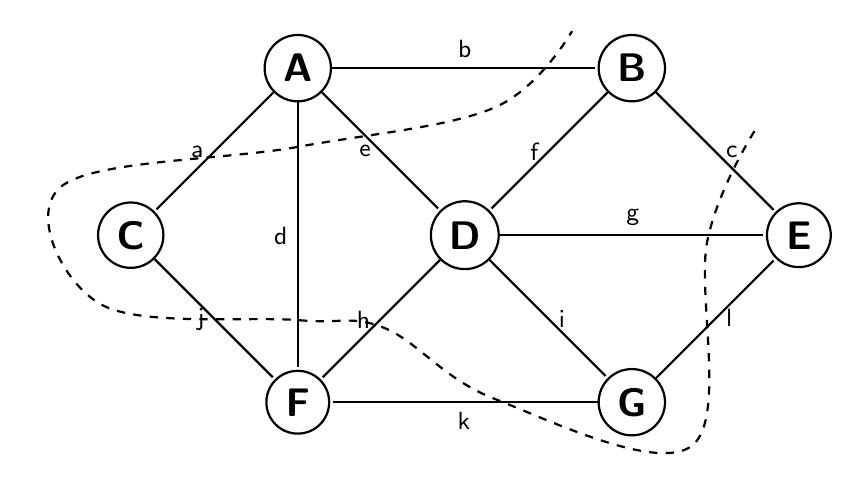
\begin{tikzpicture}[>=stealth',shorten >=1pt,auto,node distance=3cm,
                    thick,main node/.style={circle,draw,font=\sffamily\Large\bfseries}]

                    \node[main node] (A) {A};
                    \node[main node] (D) [below right of=A]{D};
                    \node[main node] (B) [above right of=D]{B};
                    \node[main node] (C) [below left of=A]{C};
                    \node[main node] (E) [below right of=B]{E};
                    \node[main node] (F) [below left of=D]{F};
                    \node[main node] (G) [below right of=D]{G};

                    \path[every node/.style={font=\sffamily\small}]
                    (A) edge node [left] {a} (C)
                    edge node [left] {d} (F)
                    edge node [left] {e} (D)
                    edge node [above] {b} (B)
                    (B) edge node [left] {f} (D)
                    edge node [right] {c} (E)
                    (C) edge node [left] {j} (F)
                    (D) edge node [above] {g} (E)
                    edge node [right] {i} (G)
                    edge node [left] {h} (F)
                    (G) edge node [below] {k} (F)
                    edge node [right] {l} (E);

                    %\draw[help lines] (-3,-5) grid (7,1);

                    \draw [black,dashed] plot [smooth,tension=0.6,looseness=4] coordinates {
                        (5.8,-0.8) 
                        (5.2,-2.2) 
                        (5,-4.8) 
                        (2.5,-4.2)
                        (1.1,-3.3)
                        (0,-3.2)
                        (-2.5,-3)
                        (-3,-1.5)
                        (0,-1)
                        (2.5,-0.5)
                        (3.5,0.5)};
                \end{tikzpicture}
            \end{center}
            \caption{Showing the Max Cut given by $s_1 = \{B,C,D,G\}, s_2 = \{A,E,F\}$}
            \belowcaptionskip0cm
        \end{figure}

        \pagebreak
        \textbf{All possible cuts of a 7 vertex graph.} \\
        The number of subgraphs possible for any given graph
        is defined as $2^{n} - 2$ but we only need half of 
        theses as changing the order of the variables does 
        not produce any new cuts.
        \begin{multicols}{2}
            \begin{tabular}{l l | }
                $\{B,C,D,E,F,G\}$ &$\{A\}$ \\
                $\{A,C,D,E,F,G\}$ &$\{B\}$ \\
                $\{C,D,E,F,G\}$ &$\{A,B\}$ \\
                $\{A,B,D,E,F,G\}$ &$\{C\}$ \\
                $\{B,D,E,F,G\}$ &$\{A,C\}$ \\
                $\{A,D,E,F,G\}$ &$\{B,C\}$ \\
                $\{D,E,F,G\}$ &$\{A,B,C\}$ \\
                $\{A,B,C,E,F,G\}$ &$\{D\}$ \\
                $\{B,C,E,F,G\}$ &$\{A,D\}$ \\
                $\{A,C,E,F,G\}$ &$\{B,D\}$ \\
                $\{C,E,F,G\}$ &$\{A,B,D\}$ \\
                $\{A,B,E,F,G\}$ &$\{C,D\}$ \\
                $\{B,E,F,G\}$ &$\{A,C,D\}$ \\
                $\{A,E,F,G\}$ &$\{B,C,D\}$ \\
                $\{E,F,G\}$ &$\{A,B,C,D\}$ \\
                $\{A,B,C,D,F,G\}$ &$\{E\}$ \\
                $\{B,C,D,F,G\}$ &$\{A,E\}$ \\
                $\{A,C,D,F,G\}$ &$\{B,E\}$ \\
                $\{C,D,F,G\}$ &$\{A,B,E\}$ \\
                $\{A,B,D,F,G\}$ &$\{C,E\}$ \\
                $\{B,D,F,G\}$ &$\{A,C,E\}$ \\
                $\{A,D,F,G\}$ &$\{B,C,E\}$ \\
                $\{D,F,G\}$ &$\{A,B,C,E\}$ \\
                $\{A,B,C,F,G\}$ &$\{D,E\}$ \\
                $\{B,C,F,G\}$ &$\{A,D,E\}$ \\
                $\{A,C,F,G\}$ &$\{B,D,E\}$ \\
                $\{C,F,G\}$ &$\{A,B,D,E\}$ \\
                $\{A,B,F,G\}$ &$\{C,D,E\}$ \\
                $\{B,F,G\}$ &$\{A,C,D,E\}$ \\
                $\{A,F,G\}$ &$\{B,C,D,E\}$ \\
                $\{F,G\}$ &$\{A,B,C,D,E\}$ \\
            \end{tabular}
            \begin{tabular}{l l}
                $\{A,B,C,D,E,G\}$ &$\{F\}$ \\
                $\{B,C,D,E,G\}$ &$\{A,F\}$ \\
                $\{A,C,D,E,G\}$ &$\{B,F\}$ \\
                $\{C,D,E,G\}$ &$\{A,B,F\}$ \\
                $\{A,B,D,E,G\}$ &$\{C,F\}$ \\
                $\{B,D,E,G\}$ &$\{A,C,F\}$ \\
                $\{A,D,E,G\}$ &$\{B,C,F\}$ \\
                $\{D,E,G\}$ &$\{A,B,C,F\}$ \\
                $\{A,B,C,E,G\}$ &$\{D,F\}$ \\
                $\{B,C,E,G\}$ &$\{A,D,F\}$ \\
                $\{A,C,E,G\}$ &$\{B,D,F\}$ \\
                $\{C,E,G\}$ &$\{A,B,D,F\}$ \\
                $\{A,B,E,G\}$ &$\{C,D,F\}$ \\
                $\{B,E,G\}$ &$\{A,C,D,F\}$ \\
                $\{A,E,G\}$ &$\{B,C,D,F\}$ \\
                $\{E,G\}$ &$\{A,B,C,D,F\}$ \\
                $\{A,B,C,D,G\}$ &$\{E,F\}$ \\
                $\{B,C,D,G\}$ &$\{A,E,F\}$ \\
                $\{A,C,D,G\}$ &$\{B,E,F\}$ \\
                $\{C,D,G\}$ &$\{A,B,E,F\}$ \\
                $\{A,B,D,G\}$ &$\{C,E,F\}$ \\
                $\{B,D,G\}$ &$\{A,C,E,F\}$ \\
                $\{A,D,G\}$ &$\{B,C,E,F\}$ \\
                $\{D,G\}$ &$\{A,B,C,E,F\}$ \\
                $\{A,B,C,G\}$ &$\{D,E,F\}$ \\
                $\{B,C,G\}$ &$\{A,D,E,F\}$ \\
                $\{A,C,G\}$ &$\{B,D,E,F\}$ \\
                $\{C,G\}$ &$\{A,B,D,E,F\}$ \\
                $\{A,B,G\}$ &$\{C,D,E,F\}$ \\
                $\{B,G\}$ &$\{A,C,D,E,F\}$ \\
                $\{A,G\}$ &$\{B,C,D,E,F\}$ \\
                $\{G\}$ &$\{A,B,C,D,E,F\}$ \\
            \end{tabular}
        \end{multicols}
    \end{quoting}

    b) Design a greedy algorithm to solve the Max-Cut problem. As part of
    your solution, you must state your greedy criteria. Further, show your algorithm
    in a concise but clear pseudo-code. You must explain in detail each line of the
    pseudo-code and show how to implement the algorithm so that it has the best
    possible time complexity. \\

    \begin{quoting}

        This algorithm initially randomly generates a subset of the graph $G$.
        From there it will choose the verticies with the highest "internal"
        degree. If the cut is improved by swapping the verticie into the other
        sub set it will accept that change. \\

        \textit{Internal degree} is the number of edges excluding any that have
        been removed by the cut. \\

        Discussion on implementation of this algorithm follows the pesudo code.

        \begin{algorithm}[H]
            \begin{algorithmic}[1]
                \Function{MaxCut}{$G, V, E$}
                \State{} $subSet = \emptyset$ \Comment{Declare a variable to store the subset we will be checking.}
                \State{} $innerDegree = \emptyset$ \Comment{A variable to store our calculated inner degree.}

                \State{} $subSet = \Call{Randomize-Sets}{V}$ \Comment{Split the vertex's into a random pair of subsets.} \\

                \For{each $vertex$ in $V$} \Comment{For each vertex in the graph}
                    \For{each $vertex.Adj$ as $edge$} \Comment{For each connected node of that vertex.}
                        \If{\Call{In-Set}{$vertex, subSet$} $=$ \Call{In-Set}{$edge, subSet$}} \Comment{If they are in the same subset}
                            \State{} $innerDegre.vertex = innerDegree.vertex + 1$ \Comment{Increment innerDegree}
                        \EndIf{}
                    \EndFor{}
                \EndFor{} \\

                \For{each $vertex$ within $innerDegree$ in descending order} \Comment{The greedy condition}
                \State{} $oldSubSet = subSet$ \Comment{Keep track of last known cut}
                    \State{} $curCut = \Call{calculateCut}{}$

                    \If{$\Call{inSet}{vertex, subSet}$}
                        \State{} $S = S - \{vertex\}$ \Comment{Remove the current vertex from the subset}
                    \Else{}
                        \State{} $S = S \cup \{vertex\}$ \Comment{Add the current vertex to the subset}
                    \EndIf{} \\

                    \If{$\Call{calculateCut}{} > curCut$} \Comment{If we found a larger cut, save it}
                        \State{} curCut = \Call{calculateCut}{} \Comment{Update the highest found cut}
                    \Else{}
                        \State{} $subSet = oldSubSet$ \Comment{We haven't found a larger cut revert the changes}
                    \EndIf{}
                \EndFor{} \\
                \EndFunction{}
            \end{algorithmic}
            \caption{Greedy algorithm to solve the MaxCut Problem}
        \end{algorithm}

        
        \begin{algorithm}[H]
            \begin{algorithmic}[1]
                \Function{Randomize-Sets}{$V$}

                    \State{}$subSet = \emptyset$ \Comment{Create an empty set to store our output} \\

                    \For{each $i$ to $|V|$ increment by 1} \Comment{For each node in the graph}
                        \State{}$randNumber = $[Random number between 0 and 1 (inc.)]
                        \If{$randNumber\,\%\,2 = 1$} \Comment{50\% change of being selected for the subset}
                            \State{}$subSet = subSet \cup \{V[i]\}$
                        \EndIf{}
                    \EndFor{} \\

                    \State{}\Return{$subSet$}

                \EndFunction{}
            \end{algorithmic}
            \caption{Randomly selects and puts vertices into a subgraph}
        \end{algorithm}

        \pagebreak
        \begin{center}
            \textit{In-Set} when expressed using set logic seems very trivial,
            however when implementing it either a while loop or linked lists 
            will be required and thus it's useful to extract the code into 
            it's own function. \\
        \end{center}

        \begin{algorithm}[H]
            \begin{algorithmic}[1]
                \Function{In-Set}{$v, subSet$}

                \If{$v \in subSet$} 
                        \State{}\Return{true}
                    \Else{}
                        \State{}\Return{false}
                    \EndIf{}

                \EndFunction{}
            \end{algorithmic}
            \caption{Checks if a vertex $v$ is contained in $subSet$}
        \end{algorithm}
        
        \begin{algorithm}[H]
            \begin{algorithmic}[1]
                \Function{Calculate-Cut}{$V, subSet$}

                    \State{}$cut = 0$

                    \For{each vertex $v \in v$}

                        \For{each edge $e \in v.Adj$}
                            \If{$\Call{In-Set}{v, subSet} \not= \Call{In-Set}{e, subSet}$}  \Comment{Checks if nodes are in different sets}
                                \State{}$cut = cut + 1$ \Comment{Given at most two subSets we only need one condition}

                                \State{}$e.Adj = e.Adj - {v}$ \Comment{Remove the inverse of the path to prevent double counts}
                            \EndIf
                        \EndFor

                    \EndFor

                \EndFunction{}
            \end{algorithmic}
            \caption{Counts the number of edges broken by a specific cut.}
        \end{algorithm}
    \end{quoting}

    \textbf{Max Cut Implementation} \\
    \begin{quoting}
       This algorithm uses multiple sets of vertices to try and generate the
       Max Cut of a graph G. The pesudo code that is shown is using set logic
       to describe opperations that are being performed on these sets. Because
       of this the code looks far simplier than it would be finally implemented.
       There are two main ways that this information can be represented in the final
       implmentation, each having a few trade offs which need to be weighed up
       relative to the situation. \\
       
       The first and simplest method is to use arrays, almost all programming
       languages have some form of arrays as a primative data type. Arrays do
       have a downside with respect to the time complexity of opperations on
       them. In memory arrays are generally represented as a single chunk,
       because of this adding or removing from anywhere but the end of the
       array requires shuffling all the other pieces of information around.
       Shuffling information around has a time complexity of $O(n)$ as the
       worst case senario involves moving the entire arrary.  With in small
       cases, much like the problem we have been given, this is not an issue as
       the input size is low ($n = 7$). But for very large values of $n$ it can
       become very troublesome as we do several additions and deletions per
       input. \\

       Another option is linked lists, these aren't usually an existing datatype
       in most programming languages but can be made by bolting together various
       other data types. Linked lists unlike arrays are represented as induvidual
       blocks in memory with each storing a reference to the next node in the list.
       As a result of this, we are able to easily add and delete elements without
       having to shuffle things out of the way. The trade off for this is the
       extra space that is required to store the references between each node.

       There are several variations of linked lists which store different
       references to try and bring down the time complexity. The traditional
       linked list has references going in one directions with each only
       pointing to the next node. While this does give us $O(1)$ complexity for
       insertion and deletion we will still require $O(n)$ searching for each
       of these operstions. We also aren't able to get back to the start of the
       list once we have started traversing it. A good variation of the linked
       list for this algorithm would have each node store the pointer to the
       next node along with a pointer to the head and tail node (The very
       first/last in the list). This would result in $O(1)$ insertion and 
       deletion, assuming we have a refference to the node already. \\

       By maintaining the head, tail and next references we are able to cut
       down much of the time complexity of our set operations. \\

       \begin{center}
           \begin{tabular}{l | c | c}

               Operation & Array & Linked List \\
               \hline
               Randomize-Set & $O(|V|)$ & $O(|V|)$ \\
               In-Set & $O(|V|)$ & $O(1)$ \\
               Calculate-Cut & $O(|V|^{2}.|E|)$ & $O(|V|.|E|)$ \\

           \end{tabular}
       \end{center}

       Linked lists look like the obvious choice, but you must also take into
       consideration what platform the final program will need to perform on.
       If memory is an issue and it is acceptable to have some delays in time
       then arrays are definitalty a good choice. However in the majority of
       situations the computer running the program is going to have Gigabytes
       of memory and it's unlikely this algorithm will use all of that. \\
   \end{quoting}

   c) Use your algorithm in part b) to generate the Max-Cut of the given
   graph. Does your algorithm generate an optimal result? \\

   \begin{quoting}

       No, my algorithm will not always generate the optimal result, it's
       unlikely for most greedy algorithms to generate the global optimal
       result given they only look at the local level.  \\

       This is part of the reason why I decided to use a random component
       within this algoirthm, if the algorithm is presented with a graph
       which has some tricky choices simply running it again may present
       to the algorithm again in an arrangement it can handle. The MaxCut
       problem solutions can easliy be ranked by the \textit{CalculateCut}
       function and so running this algorithm several time and taking the
       best solution is not a problem. \\

       Below is an output from running an implementation of my algorithm
       once. You can see in the first line even though the cut presented
       initially was not great, the algorithm still managed to generate a
       cut of a size 1 smaller than the optimal solution.

       \VerbatimInput{singleRun}

   \end{quoting}

   d) Give a counter example to show that your greedy algorithm does not
   always generate an optimal result. \\

   \begin{quoting}

       My algorithm particually falls down when the subsets aren't even,
       take the example of $s_1 = {G}, s_2 = {A, B, C, D, E, F}$, you can
       see this is the worst possible case for the algoirthm given the is
       absoultely no internal links within $s_1$ and within $s_2$ they are
       basically all interlinked. What will end up happening in this situation
       is the sets will likely reverse and the cut we get at the end is simply
       the randomly generated one at the start.

   \end{quoting}



\end{homeworkProblem}

\end{document}
